% The real graph of x^5-4x+2, with its three crossings.
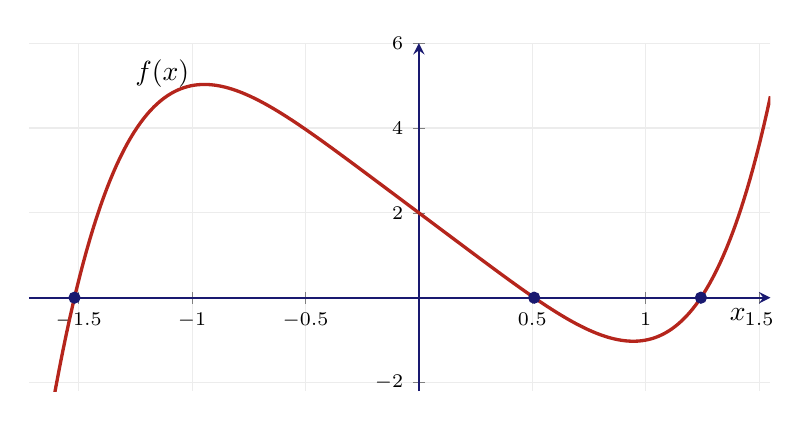
\begin{tikzpicture}
\begin{axis}[
 width=11cm,height=6cm,xmin=-1.72,xmax=1.55,ymin=-2.2,ymax=6,
 axis lines=middle,axis line style={MidnightBlue,thick},
 xlabel={$x$},ylabel={$f(x)$},xlabel style={at={(axis description cs:0.98,0.22)},anchor=east},
 ylabel style={at={(axis description cs:0.18,0.98)},anchor=north},
 xtick={-1.5,-1,-.5,0,.5,1,1.5},ytick={-2,0,2,4,6},
 tick label style={font=\scriptsize},grid=both,
 major grid style={draw=gray!15},minor grid style={draw=gray!7},
 clip=true]
\addplot[domain=-1.72:1.55,samples=220,very thick,BrickRed] {x^5-4*x+2};
\addplot[only marks,mark=*,mark size=2pt,MidnightBlue] coordinates {
(-1.51851215,0) (0.50849948,0) (1.24359639,0)};
\end{axis}
\end{tikzpicture}
